
\chapter{Circle of curvature. Center of Curvature.}
\label{ch:14}


%116. 
\section{Circle of curvature}
\label{sec:116}

Center of curvature\footnote{Sometimes called the 
{\it osculating circle}. The circle of curvature was defined from 
another point of view in \S \ref{sec:104}.}. If a circle be drawn 
through three points $P_0$, $P_1$, $P_2$ on a plane curve, and if 
$P_1$ and $P_2$ be made to approach $P_0$ along the curve as a 
limiting position, then the circle will in general approach in 
magnitude and position a limiting circle called the circle of 
curvature of the curve at the point $P_0$. The center of this 
circle is called the {\it center of curvature}.
\index{center of curvature}

\begin{figure}[h!]
%\begin{tabular}{cc}
\begin{minipage}{\textwidth}
\begin{center}
%\vspace{1.0 cm}
%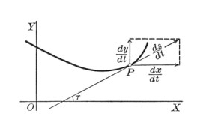
\includegraphics[height=3cm,width=6cm]{two-rates.eps}
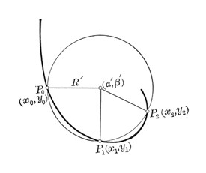
\includegraphics[height=4cm,width=6cm]{circle-of-curvature.eps}
\end{center}
\end{minipage}
%\caption{Scan of Granville's graphic of the derivative the arc length.}
\caption{Geometric visualization of the circle of curvature.}
\label{fig:circle-of-curvature}
\end{figure}

Let the equation of the curve be

\begin{equation}
%(1) 
\label{eqn:116-1}
y = f(x);
\end{equation}
and let $x_0$, $x_1$, $x_2$ be the abscissas of the points 
$P_0$, $P_1$, $P_2$ respectively, $(\alpha',\alpha')$ the coordinates 
of the center, and $R'$ the radius of the circle passing through 
the three points. Then the equation of the circle is

\[
 (x-\alpha')^2 + (y-\beta')^2 = (R')^2;
\]
and since the coordinates of the points $P_0$, $P_1$, $P_2$ 
must satisfy this equation, we have

\begin{equation}
%(2) 
\label{eqn:116-2}
\begin{cases} (x_0 - \alpha')^2 + (y_0 -\beta')^2 - R'^2 = 0, \\ 
(x_1 - \alpha')^2 + (y_1 - \beta')^2 -(R')^2 = 0, \\ 
(x_2 - \alpha')^2 + (y_2 - \beta')^2 -(R')^2 = 0.
\end{cases}
\end{equation}
Now consider the function of $x$ defined by

\[
    F(x) = (x-\alpha')^2 + (y-\beta')^2 - (R')^2,
\]
in which $y$ has been replaced by $f(x)$ from (\ref{eqn:116-1}).

Then from equations (\ref{eqn:116-2}) we get

\[
    F(x_0) = 0,\ F(x_1) = 0,\ F(x_2) = 0.
\]
Hence, by Rolle's Theorem (\S \ref{sec:105}), $F'(x)$ must vanish 
for at least two values of $x$, one lying between $x_0$ and $x_1$, 
say $x'$, and the other lying between $x_1$ and $x_2$ say $x''$; that is,

\[
    F'(x') = 0,F'(x'') = 0.
\]
Again, for the same reason, $F''(x)$ must vanish for some value 
of $x$ between $x'$ and $x''$, say $x_3$; hence

\[
    F''(x_3) = 0.
\]
Therefore the elements $\alpha'$, $\beta'$, $R'$ of the circle 
passing through the points $P_0$, $P_1$, $P_2$ must satisfy the three 
equations

\[
    F(x_0) = 0,\ F'(x') = 0,\ F''(x_3) = 0. 
\]
Now let the points $P_1$ and $P_2$ approach $P_0$ as a limiting 
position; then $x_1$, $x_2$, $x'$, $x''$, $x_3$ will all approach 
$x_0$ as a limit, and the elements $\alpha$, $\beta$, $R$ of the 
osculating circle are therefore determined by the three equations

\[
    F(x_0) = 0,\ F'(x_0) = 0,\ F''(x_0) = 0;
\]
or, dropping the subscripts, which is the same thing,

\begin{equation}
%(A) 
\label{eqn:116A}
(x - \alpha)^2 + (y -\beta)^2 = R^2
\end{equation}

\begin{equation}
%(B) 
\label{eqn:116B}
(x - \alpha) + (y -\beta)\frac{dy}{dx} = 0,
\end{equation}
differentiating (\ref{eqn:116A}).

\begin{equation}
%(C) 
\label{eqn:116C}
1 + \left( \frac{dy}{dx} \right)^2 + (y - \beta) \frac{d^2 y}{dx^2} = 0, 
\end{equation}
differentiating (\ref{eqn:116B}).
Solving (\ref{eqn:116B}) and (\ref{eqn:116C}) for 
$x-\alpha$ and $y-\beta$, we get 
$\left( \frac{d^2 y}{dx^2} \ne 0 \right)$,

\begin{equation}
%(D) 
\label{eqn:116D}
\begin{cases} 
x - \alpha = \frac{\frac{dy}{dx} 
\left[ 1 + \left( \frac{dy}{dx} \right)^2 \right]}{\frac{d^2 y}{dx^2}} \\ 
y - \beta 
= -\frac{1 + \left( \frac{dy}{dx} \right)^2}{\frac{d^2 y}{dx^2}};
\end{cases}
\end{equation}
hence the coordinates of the center of curvature are

\begin{equation}
%(E) 
\label{eqn:116E}
\alpha = x - \frac{\frac{dy}{dx} 
\left[1 + \left( \frac{dy}{dx} \right)^2 \right]}{\frac{d^2 y}{dx^2}}; 
\beta = y + \frac{1 + \left( \frac{dy}{dx} \right)^2}{\frac{d^2 y}{dx^2}}. 
\left( \frac{d^2 y}{dx^2} \ne 0 \right)
\end{equation}

Substituting the values of $x-\alpha$ and $y-\beta$ from 
(\ref{eqn:116D}) in (\ref{eqn:116A}), and solving for $R$, we get

\[
    R = \pm \frac{ \left[ 1 + 
\left( \frac{dy}{dx} \right)^2 \right]^{\frac{3}{2}} }{ \frac{d^2 y}{dx^2} },
\]
which is identical with (\ref{eqn:103-42}), [\S \ref{sec:103}]. 
Hence

\begin{theorem}
The radius of the circle of curvature equals the radius of curvature.
\end{theorem}


%117. 
\section{Second method for finding center of curvature}
\label{sec:117}

Here we shall make use of the definition of circle of curvature 
given in \S \ref{sec:104}. Draw a figure showing the tangent line, 
circle of curvature, radius of curvature, and center of curvature 
$(\alpha, \beta)$ corresponding to the point $P(x,y)$ on the curve. Then

\[
    \alpha = OA = OD - AD = OD - BP = x - BP,
\]
\[
\beta = AC = AB + BC = DP + BC = y + BC.
\]
But $BP = R\sin \tau$, $BC = R\cos \tau$. Hence

\begin{equation}
%(A) 
\label{eqn:117-A}
\alpha = x -R\sin \tau,\ \ \ \ \beta = y + R\cos \tau.
\end{equation}

From (\ref{eqn:90-29}) [\S \ref{sec:90}], and (\ref{eqn:103-42})
[\ref{sec:103}],

\[
\sin \tau 
= \frac{ \frac{dy}{dx} }{ \left[ 1 
+ \left( \frac{dy}{dx} \right)^2 \right]^{\frac{1}{2}} }, 
\]
\[
\cos \tau 
= \frac{1}{\left[ 1 + 
\left( \frac{dy}{dx} \right)^{\frac{1}{2}} \right]^{\frac{1}{2}}}, 
\]
\[
R = \frac{ \left[ 1 
+ \left( \frac{dy}{dx} \right)^2 \right]^{\frac{3}{2}} }{ \frac{d^2 y}{dx^2} }
\]
Substituting these back in (\ref{eqn:117-A}), we get

\begin{equation}
%(50) 
\label{eqn:117-50}
\alpha = x - \frac{ \frac{dy}{dx}\left[ 1 + \left( \frac{dy}{dx} \right)^2 \right] }{\frac{d^2 y}{dx^2}}; 
\ \ \ \ 
\beta = y + \frac{1 + \left( \frac{dy}{dx} \right)^2}{\frac{d^2 y}{dx^2}}.
\end{equation}
From Lemma \ref{lemma:85-23} [\S \ref{sec:85}], we know that at a 
point of inflection (as Q in Figure \ref{fig:circle-of-curvature2})

\[
    \frac{d^2 y}{dx^2} = 0.
\]

\begin{figure}[h!]
%\begin{tabular}{cc}
\begin{minipage}{\textwidth}
\begin{center}
%\vspace{1.0 cm}
%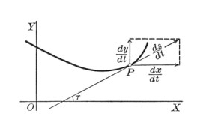
\includegraphics[height=3cm,width=6cm]{two-rates.eps}
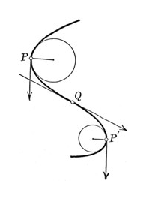
\includegraphics[height=4.5cm,width=4cm]{circle-of-curvature2.eps}
\end{center}
\end{minipage}
%\caption{Scan of Granville's graphic of the derivative the arc length.}
\caption{Geometric visualization of a change in direction.}
\label{fig:circle-of-curvature2}
\end{figure}

\noindent
Therefore, by (\ref{eqn:102-40}) [\S \ref{sec:102}], the curvature 
$K = 0$; and from (\ref{eqn:103-42}) [\S \ref{sec:103}], 
and (\ref{eqn:117-50}) [\S \ref{sec:117}], we see that in general 
$\alpha$, $\beta$, $R$ increase without limit as the second 
derivative approaches zero. That is, if we suppose $P$ with its 
tangent to move along the curve to $P'$, at the point of 
inflection $Q$ the curvature is zero, the rotation of the tangent 
is momentarily arrested, and as the direction of rotation changes, 
the center of curvature moves out indefinitely and the radius 
of curvature becomes infinite.


\begin{example}
Find the coordinates of the center of curvature of the 
parabola $y^2 = 4px$ corresponding (a) to any point on the curve; 
(b) to the vertex.

Solution. $\frac{dy}{dx} = \frac{2p}{y}$; 
$\frac{d^2 y}{dx^2} = -\frac{4p^2}{y^3}$.

(a) Substituting in (\ref{eqn:116E}) [\S \ref{sec:116}],

\[
    \alpha = x + \frac{y^2 + 4 p^2}{y^2} \cdot \frac{2p}{y} 
\cdot \frac{y^3}{4 p^2} = 3x + 2p.
\]
\[
    \beta = y - \frac{y^2 + 4 p^2}{y^2} \cdot \frac{y^3}{4 p^2} 
= -\frac{y^3}{4 p ^2}.
\]
Therefore $\left( 3x + 2p, -\frac{y^3}{4 p^2} \right)$ 
is the center of curvature corresponding to any point on the curve.

(b) $(2p,0)$ is the center of curvature corresponding to the vertex 
$(0, 0)$.
\end{example}

%118. 
\section{Center of curvature}
\label{sec:118}

The limiting position of the intersection of normals at neighboring 
points. Let the equation of a curve be

\begin{equation}
%(A) 
\label{eqn:118A}
y = f(x).
\end{equation}

\begin{figure}[h!]
%\begin{tabular}{cc}
\begin{minipage}{\textwidth}
\begin{center}
%\vspace{1.0 cm}
%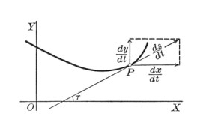
\includegraphics[height=3cm,width=6cm]{two-rates.eps}
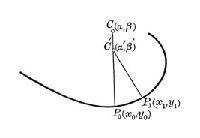
\includegraphics[height=4cm,width=6cm]{circle-of-curvature3.eps}
\end{center}
\end{minipage}
%\caption{Scan of Granville's graphic of the derivative the arc length.}
\caption{Geometric visualization of the center of curvature.}
\label{fig:circle-of-curvature3}
\end{figure}
The equations of the normals to the curve at two neighboring 
points $P_0$ and $P_1$ are (using (\ref{eqn:65-2}) [\S \ref{sec:65}]),

\[
    (x_0 - X) + (y_0 - Y) \frac{dy_0}{dx_0} = 0,
\ \ \ \ 
    (x_1 - X) + (y_1 - Y) \frac{dy_1}{dx_1} = 0.
\]
If the normals intersect at $C'(\alpha',\beta')$, the 
coordinates of this point must satisfy both equations, giving

\begin{equation}
%(B) 
\label{eqn:118B}
\begin{cases}
(x_0 - \alpha') + (y_0 - \beta) \frac{dy_0}{dx_0} = 0, \\ 
(x_1 - \alpha') + (y_1 - \beta') \frac{dy_1}{dx_1} = 0.
\end{cases}
\end{equation}
Now consider the function of x defined by

\[
    \phi(x) = (x - \alpha') + (y - \beta') \frac{dy}{dx},
\]
in which $y$ has been replaced by $f(x)$ from (\ref{eqn:118A}).
Then equations (\ref{eqn:118B}) show that

\[
\phi(x_0) = 0,\ \ \ \phi(x_1) = 0.
\]
But then, by Rolle's Theorem (\S \ref{sec:105}), 
$\phi'(x)$ must vanish for some value of $x$ between $x_0$ and 
$x_1$ say $x'$. Therefore $\alpha'$ and $\beta'$ are determined by the 
two equations

\[
\phi(x_0) = 0,\ \ \ \phi'(x') = 0.
\]
If now $P_1$ approaches $P_0$ as a limiting position, then 
$x'$ approaches $x_0$, giving

\[
\phi(x_0) = 0,\ \ \ \phi'(x_0) = 0.
\]  
and $C'(\alpha',\beta')$ will approach as a limiting position 
the center of curvature $C(\alpha,\beta)$ corresponding to 
$P_0$ on the curve. For if we drop the subscripts and write 
the last two equations in the form

\[
    (x - \alpha') + (y - \beta') \frac{dy}{dx} = 0,
\ \ \ \ 
1 + \left( \frac{dy}{dx} \right)^2 + (y - \beta') \frac{d^2 y}{dx^2} = 0,
\]
it is evident that solving for $\alpha'$ and $\beta'$ will 
give the same results as solving (\ref{eqn:116B}) and 
((\ref{eqn:116C}) for $\alpha$ and $\beta$. Hence we have the following 
result.

\begin{theorem}
The center of curvature $C$ corresponding to a point $P$ on a curve 
is the limiting position of the intersection of the normal 
to the curve at $P$ with a neighboring normal.
\end{theorem}


%119. 
\section{Evolutes}
\label{sec:119}

The locus of the centers of curvature of a given curve is called 
the {\it evolute} of that curve. 
\index{evolute}
Consider the circle of curvature corresponding to a point $P$ on a curve. 
If $P$ moves along the given curve, we may suppose the corresponding 
circle of curvature to roll along the curve with it, its radius 
varying so as to be always equal to the radius of curvature 
of the curve at the point $P$. The curve $CC_7$ in Figure \ref{fig:evolutes}
described by the center of the circle is the evolute of $PP_7$.

\begin{figure}[h!]
%\begin{tabular}{cc}
\begin{minipage}{\textwidth}
\begin{center}
%\vspace{1.0 cm}
%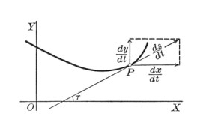
\includegraphics[height=3cm,width=6cm]{two-rates.eps}
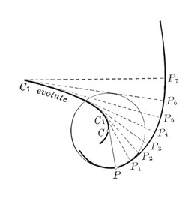
\includegraphics[height=5cm,width=6cm]{evolutes.eps}
\end{center}
\end{minipage}
%\caption{Scan of Granville's graphic of the derivative the arc length.}
\caption{Geometric visualization of an evolute.}
\label{fig:evolutes}
\end{figure}
 
\noindent
It is instructive to make an approximate construction of 
the evolute of a curve by estimating (from the shape of the 
curve) the lengths of the radii of curvature at different 
points on the curve and then drawing them in and drawing the 
locus of the centers of curvature.

Formula (\ref{eqn:116E}) %(E), p. 179 [§116], 
gives the coordinates of any 
point $(\alpha,\beta)$ on the evolute expressed in terms of the coordinates 
of the corresponding point $(x,y)$ of the given curve. But 
$y$ is a function of $x$; therefore

\[
    \alpha 
= x - \frac{ \left[ 1 + \left( \frac{dy}{dx} \right)^2 \right] \frac{dy}{dx} }{ \frac{d^2 y}{dx^2} }, 
\ \  \ \ \ \ \ \ 
\beta = y + \frac{ 1 + \left( \frac{dy}{dx} \right)^2 }{ \frac{d^2 y}{dx^2} } 
\]
give us at once the parametric equations of the evolute in 
terms of the parameter x.

To find the ordinary rectangular equation of the evolute 
we eliminate $x$ between the two expressions. No general 
process of elimination can be given that will apply in all 
cases, the method to be adopted depending on the form of the 
given equation. In a large number of cases, however, the 
student can find the rectangular equation of the evolute by 
taking the following steps:

General directions for finding the equation of the evolute in 
rectangular coordinates.

\begin{itemize}
\item
FIRST STEP. Find $\alpha,\beta$ from (\ref{eqn:117-50}). %(50), p. 180 [§117].

\item
SECOND STEP. Solve the two resulting equations for $x$ and $y$ 
in terms of $\alpha$ and $\beta$.

\item
THIRD STEP. Substitute these values of $x$ and $y$ in the given 
equation. This gives a relation between the variables 
$\alpha$ and $\beta$ which is the equation of the evolute.
\end{itemize}

\begin{example}
Find the equation of the evolute of the parabola $y^2 = 4px$.

\begin{figure}[h!]
%\begin{tabular}{cc}
\begin{minipage}{\textwidth}
\begin{center}
%\vspace{1.0 cm}
%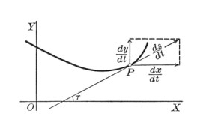
\includegraphics[height=3cm,width=6cm]{two-rates.eps}
\includegraphics[height=4cm,width=6cm]{evolute-of-parabola.eps}
\end{center}
\end{minipage}
%\caption{Scan of Granville's graphic of the derivative the arc length.}
\caption{Evolute of a parabola.}
\label{fig:evolute-of-parabola}
\end{figure}
 

Solution. 	
$\frac{dy}{dx} 	=\ \frac{2p}{y}, \frac{d^2 y}{dx^2} = -\frac{4p^2}{y^3}$.

First step. 	
$\alpha= 3x + 2p$, $\beta = -\frac{y^3}{4p^2}$.

Second step. 	
$x= \frac{\alpha - 2p}{3}$, $y = -(4p^2 \beta)^{\frac{1}{3}}$.

Third step 	
$(4p^2 \beta)^{\frac{2}{3}} = 4p \left( \frac{\alpha - 2p}{3} \right)$;  
or, $p\beta^2\frac{4}{27} (\alpha - 2p)^3$.

Remembering that $\alpha$ denotes the abscissa and $\beta$ the 
ordinate of a rectangular system of coordinates, 
we see that the evolute of the parabola $AOB$ is the semi-cubical 
parabola $DC'E$; the centers of curvature for $O$, $P$, $P_1$, $P_2$ 
being at $C'$, $C$, $C_1$, $C_2$ respectively.
\end{example}

\begin{example}
{\rm
Find the equation of the evolute of the parabola $b^2x^2+a^2y^2 = a^2b^2$.

\begin{figure}[h!]
%\begin{tabular}{cc}
\begin{minipage}{\textwidth}
\begin{center}
%\vspace{1.0 cm}
%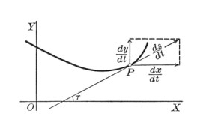
\includegraphics[height=3cm,width=6cm]{two-rates.eps}
\includegraphics[height=4cm,width=6cm]{evolute-of-ellipse.eps}
\end{center}
\end{minipage}
%\caption{Scan of Granville's graphic of the derivative the arc length.}
\caption{Evolute of an ellipse.}
\label{fig:evolute-of-an-ellipse}
\end{figure}

Solution. 	
$\frac{dy}{dx} 	= -\frac{b^2 x}{a^2 y}$, 
$\frac{d^2 y}{dx^2} = -\frac{b^4}{a^2 y^3}$.

First step. $\alpha = \frac{(a^2 - b^2)x^3}{a^4}$,
$\beta 	= -\frac{(a^2 - b^2)y^3}{b^4}$.

Second step. 	
$x 	= \left( \frac{a^4 \alpha}{a^2 - b^2} \right)^{frac{1}{3}}$,
$y 	= -\left( \frac{b^4 \beta}{a^2 - b^2} \right)^{\frac{1}{3}}$.

Third step. $(a\alpha)^{\frac{2}{3}} + (b\beta)^{\frac{2}{3}} 
= (a^2 - b^2)^{\frac{2}{3}}$, the equation of the evolute 
$EHE'H'$ of the ellipse $ABA'B'$, $E$, $E'$, $H'$, $H$ are the 
centers of curvature corresponding to the points $A$, $A'$, $B$, $B'$, 
on the curve, and $C$, $C'$, $C''$ correspond to the points 
$P$, $P'$, $P''$.
}
\end{example}

When the equations of the curve are given in parametric form, 
we proceed to find $\frac{dy}{dx}$ and $\frac{d^2 y}{dx^2}$, 
as in \S \ref{sec:103}, from %on p. 160 [§103], 

\begin{equation}
\label{eqn:119A}
%(A) 	
\frac{dy}{dx} 
= \frac{ \frac{dy}{dt} }{ \frac{dx}{dt} }, 
\ \ \ \ \ \ \ 
\frac{d^2 y}{dx^2} 
= \frac{ \frac{dx}{dt} \frac{d^2 y}{dt^2} 
- \frac{dy}{dt} \frac{d^2 x}{dt^2} }{ \left( \frac{dx}{dt} \right)^3 }
\end{equation}
and then substitute the results in 
formulas (\ref{eqn:117-50}). %(50), p. 180 [§117]. 
This gives the parametric equations of the evolute in terms 
of the same parameter that occurs in the given equations.

\begin{example}
{\rm
The parametric equations of a curve are

\begin{equation}
\label{eqn:119B}
%(B) 	
x = \frac{t^2 + 1}{4}, \ \ \ \ \ \ 
y = \frac{t^3}{6}.
\end{equation}
Find the equation of the evolute in parametric form, 
plot the curve and the evolute, find the radius of curvature 
at the point where $t = 1$, and draw the corresponding circle of curvature.

Solution. 	
$\frac{dx}{dt} = \frac{t}{2}$, $\frac{d^2 x}{dt^2} = \frac{1}{2}$,
$\frac{dy}{dt} = \frac{t^2}{2}$, $\frac{d^2 y}{dt^2} = t$.
Substituting in above formulas (\ref{eqn:119A}) %(A) 
and then in (\ref{eqn:117-50}), %(50), p. 180 [§117], 
gives

\begin{equation}
\label{eqn:119C}
%(C) 	
\alpha = \frac{1 - t^2 - 2t^4}{4}, \ \ \ \ \ \ 
\beta = \frac{4t^3 + 3t}{6},
\end{equation}
the parametric equations of the evolute. Assuming values of 
the parameter $t$, we calculate $x$, $y$; $\alpha, \beta$
from (\ref{eqn:119B}) and (\ref{eqn:119C}).
Now plot the curve and its evolute.

\begin{figure}[h!]
%\begin{tabular}{cc}
\begin{minipage}{\textwidth}
\begin{center}
%\vspace{1.0 cm}
%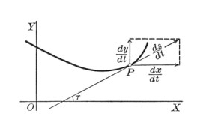
\includegraphics[height=3cm,width=6cm]{two-rates.eps}
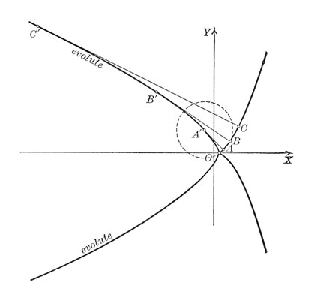
\includegraphics[height=4cm,width=6cm]{evolute-parametric-example.eps}
\end{center}
\end{minipage}
%\caption{Scan of Granville's graphic of the derivative the arc length.}
\caption{Evolute of an parametric curve.}
\label{fig:evolute-parametric-example}
\end{figure}

\noindent
The point $(\frac{1}{4}, 0)$ is common to the given curve 
and its evolute. The given curve (a semi-cubical parabola) lies 
entirely to the right and the evolute entirely to the left of 
$x = \frac{1}{4}$.

The circle of curvature at $A= (\frac{1}{2}, \frac{1}{6})$, 
where $t = 1$, will have its center at 
$A'= (-\frac{1}{2}, -\frac{7}{6})$ on the evolute and radius 
$= AA'$. To verify our work, find radius of curvature at $A$. From 
(\ref{eqn:103-42}), %(42), p. 159 [§103], 
we get

\[
R = \frac{t(1 + t^2)^{\frac{3}{2}}}{2} = \sqrt{2}, 
\]
when $t= 1$.
This should equal the distance

\[
    AA' 
= \sqrt{(\frac{1}{2} + \frac{1}{2})^2 +
(\frac{1}{6} - \frac{7}{6})^2} = \sqrt{2}.
\]
}
\end{example}

\begin{example}
\label{ex:118-cycloid}
{\rm
Find the parametric equations of the evolute of the cycloid,

\begin{equation}
\label{eqn:119C2}
%(C) 	-- there are actually two (C)'s in section 119
\begin{cases} 
x = a(t - \sin t) \\ 
y = a(1 - \cos t).
\end{cases}
\end{equation}

\begin{figure}[h!]
%\begin{tabular}{cc}
\begin{minipage}{\textwidth}
\begin{center}
%\vspace{1.0 cm}
%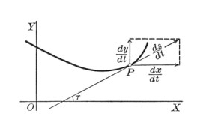
\includegraphics[height=3cm,width=6cm]{two-rates.eps}
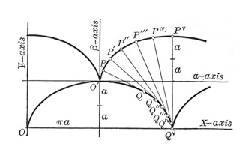
\includegraphics[height=4cm,width=6cm]{evolute-of-cycloid.eps}
\end{center}
\end{minipage}
%\caption{Scan of Granville's graphic of the derivative the arc length.}
\caption{Evolute of a cycloid.}
\label{fig:evolute-of-cycloid}
\end{figure}

\noindent
Solution. As in Example \ref{ex:103-2}, %EXAMPLE 2, p. 160 [§103], 
we get

\[
  	\frac{dy}{dx} = \frac{\sin t}{1 - \cos t}, 
\ \ \ \ \ 
\frac{d^2 y}{dx^2} = -\frac{1}{\alpha (1 - \cos t)^2}.
\]
Substituting these results in formulas (\ref{eqn:117-50}), %(50),p. 180[§117], 
we get the answer:

\begin{equation}
\label{eqn:119D}
%(D) 	
\begin{cases} 
\alpha = a(t + \sin t), \\ 
\beta = -a(1 - \cos t).
\end{cases} 
\end{equation}
}
\end{example}


\begin{remark}
{\rm
In the previous example,
if we eliminate $t$ between equations (\ref{eqn:119D}), there results 
the rectangular equation of the evolute $OO'Q^v$ referred to 
the axes $O'\alpha$ and $O'\beta$. The coordinates of $O$ with 
respect to these axes are $(-\pi a, -2a)$. Let us transform 
equations (\ref{eqn:119D}) to the new set of axes $OX$ and $OY$. Then

\[
\alpha = x -\pi a,\ \ \ \ \beta = y -2a,\ \ \ \ t = t' -\pi.
\]
Substituting in (\ref{eqn:119D}) and reducing, the 
equations of the evolute become

\begin{equation}
\label{eqn:119E}
%(E) 
\begin{cases} 
x = a(t' - \sin t'), \\ 
y = a(1 - \cos t').
\end{cases}
\end{equation}
Since (\ref{eqn:119E}) and (\ref{eqn:119C}) are identical in form, we have:
{\it The evolute of a cycloid is itself a cycloid whose 
generating circle equals that of the given cycloid.}
}
\end{remark}



%119. 
\section{Properties of the evolute}
\label{sec:120}


From (\ref{eqn:117-A}), %(A), p. 180 [§117],

\begin{equation}
\label{eqn:120-A}
%(A) 
\alpha = x - R\sin\, \tau,\ \ \ \ \ 
\beta = y + R\cos\, \tau.
\end{equation}
Let us choose as independent variable the lengths of the arc 
on the given curve; then $x$, $y$, $R$, $T$, $\alpha$,
$\beta$ are functions of $s$. Differentiating 
(\ref{eqn:120-A}) with respect to $s$ gives

\begin{equation}
\label{eqn:120-B}
%(B) 
\frac{d\alpha}{ds} 
= \frac{dx}{ds} - R \cos \tau \frac{d\tau}{ds} - \sin \tau \frac{dR}{ds},
\end{equation}

\begin{equation}
\label{eqn:120-C}
%(C) 
\frac{d\beta}{ds} 
= \frac{dy}{ds} - R \sin \tau \frac{d\tau}{ds} + \cos \tau \frac{dR}{ds}.
\end{equation}
But $\frac{dx}{ds} = \cos \tau$, $\frac{dy}{ds} = \sin \tau$, from 
(\ref{eqn:90-26}); %(26) p. 134 [§90]; 
and $\frac{d\tau}{ds} = \frac{1}{R}$, from (\ref{eqn:100-38}) 
and (\ref{eqn:101-39}). %, p. 156 [§100–1].

Substituting in (\ref{eqn:120-B}) and (\ref{eqn:120-C}), we obtain

\begin{equation}
\label{eqn:120-D}
%(D) 
\frac{d\alpha}{ds} 
= \cos \tau - R \cos \tau \cdot \frac{1}{R} - \sin \tau \frac{dR}{ds} 
= - \sin \tau \frac{dR}{ds},
\end{equation}
and
\begin{equation}
\label{eqn:120-E}
%(E) 
\frac{d\beta}{ds} 
= \sin \tau - R \sin \tau \cdot \frac{1}{R} + \cos \tau \frac{dR}{ds} 
= \cos \tau \frac{dR}{ds}.
\end{equation}
Dividing (\ref{eqn:120-E}) by (\ref{eqn:120-D}) gives

\begin{equation}
\label{eqn:120-F}
%(F) 
\frac{d\beta}{d\alpha} 
= - \cot \tau = - \frac{1}{\tan \tau} 
= - \frac{1}{\frac{dy}{dx}}.
\end{equation}
But 
$\frac{d\beta}{d\alpha} = \tan \tau$ = slope of tangent to the 
evolute at $C$, and
$\frac{dy}{dx} = \tan \tau$ = slope of tangent to the given curve 
at the corresponding point $P(x,y)$.

Substituting the last two results in (\ref{eqn:120-F}), we get

\[
    \tan \tau' = - \frac{1}{\tan \tau}.
\]
Since the slope of one tangent is the negative reciprocal 
of the slope of the other, they are perpendicular. But a 
line perpendicular to the tangent at $P$ is a normal to the curve. Hence

{\it A normal to the given curve is a tangent to its evolute.}

Again, squaring equations (\ref{eqn:120-D}) and (\ref{eqn:120-E})
and adding, we get

\begin{equation}
\label{eqn:120-G}
%(G) 
\left( \frac{d\alpha}{ds} \right)^2 + 
\left( \frac{d\beta}{ds} \right)^2 
= \left( \frac{dR}{ds} \right)^2.
\end{equation}
But if $s'$ = length of arc of the evolute, the left-hand member 
of (\ref{eqn:120-G}) is precisely the square of $\frac{ds'}{ds}$ 
(from (\ref{eqn:34-94}), %(34) p. 141 [§94], 
where $t = s$, $s = s'$, $x = \alpha$, $y = \beta$). 
Hence (\ref{eqn:120-G}) asserts that

\[
  \left( \frac{ds'}{ds} \right)^2 
= \left( \frac{dR}{ds} \right)^2, \ \ \ \ 
\text{ or } \ \ \ \ 
\frac{ds'}{ds} = \pm \frac{dR}{ds}.
\]
That is, the radius of curvature of the given curve increases or 
decreases as fast as the arc of the evolute increases. In our 
figure this means that

\[
    P_1 C_1 - PC = \text{arc}\ CC_1.
\]
The length of an arc of the evolute is equal to the 
difference between the radii of curvature of the given curve 
which are tangent to this arc at its extremities.

Thus in Example \ref{ex:118-cycloid}, %4, p. 186 [§118], 
we observe that if we fold $Q_vP_v$ ( $= 4a$) over to the 
left on the evolute, $P_v$ will reach to $O'$, and we have:

{\it The length of one arc of the cycloid (as $OO'Q_v$) 
is eight times the length of the radius of the generating circle.
}

\section{Exercises}


Find the coordinates of the center of curvature and the 
equation of the evolute of each of the following curves. 
Draw the curve and its evolute, and draw at least one circle of curvature.

\begin{enumerate}
\item
The hyperbola $\frac{x^2}{a^2} - \frac{y^2}{b^1} = 1$. 	

Ans. 	$\alpha = \frac{(a^2 + b^2)x^3}{a^4}$, 
$\beta = -\frac{(a^2 + b^2)y^3}{b^4}$; evolute 
$(a\alpha)^{\frac{2}{3}} - (b\beta)^{\frac{2}{3}} = (a^2 + b^2)^{\frac{2}{3}}$.

\item
The hypocycloid $x^{\frac{2}{3}} + y^{\frac{2}{3}} = a^{\frac{2}{3}}$. 	  	

$\alpha = x + 3x^{\frac{1}{3}} y^{\frac{2}{3}}$, 
$\beta = y + 3 x^{\frac{2}{3}} y^{\frac{1}{3}}$;
evolute 
$(\alpha + \beta)^{\frac{2}{3}} + (\alpha - \beta)^{\frac{2}{3}} 
= 2a^{\frac{2}{3}}$.

\item
Find the coordinates of the center of curvature of the 
cubical parabola $y^3 = a^2x$.

Ans. 	
$\alpha = \frac{a^4 + 15y^4}{6a^2 y}$, 
$\beta = \frac{a^4y - 9y^5}{2a^4}$.

\item
Show that in the parabola 
$x^{\frac{1}{2}} + y^{\frac{1}{2}} = a^{\frac{1}{2}}$ we 
have the relation $\alpha + \beta = 3(x + y)$.

\item
Given the equation of the equilateral hyperbola $2xy = a^2$ show that

\[
 \alpha + \beta 
= \frac{(y + x)^3}{a^2}, \alpha - \beta = \frac{(y - x)^3}{a^2}.
\]
From this derive the equation of the evolute 
$(\alpha + \beta)^{\frac{2}{3}} - (\alpha - \beta)^{\frac{2}{3}} 
= 2 a^{\frac{2}{3}}$.
\end{enumerate}

Find the parametric equations of the evolutes of the 
following curves in terms of the parameter $t$. 
Draw the curve and its evolute, and draw at least one circle of curvature.

6. The hypocycloid 
$\begin{cases} x = a \cos^3 t, 
\\ y = a \sin^3 t. \end{cases}$ 	

Ans. 	
$\begin{cases} \alpha = a \cos^3 t + 3a \cos t \sin^2 t, 
\\ \beta = 3a \cos^2 t \sin t + a \sin^3 t. \end{cases}$.

7. The curve 	
$\begin{cases} x = 3t^2, 
\\ y = 3t - t^3. \end{cases}$

Ans.
$\begin{cases} \alpha 
= \frac{3}{2} ( 1 + 2t^2 - t^4 ), \\ 
\beta = -4 t^3. \end{cases}$

8. The curve 	
$\begin{cases} x = a(\cos t + t \sin t), \\ 
y = a(\sin t - t \cos t). \end{cases}$. 

Ans. 	
$\begin{cases} \alpha = a \cos t, 
\\ \beta = a \sin t. \end{cases}$.

9. The curve 
$\begin{cases} x = 3t, 
\\ y = t^2 -6. \end{cases}$.

Ans. $\begin{cases} \alpha = -\frac{4}{3} t^3, \\ 
\beta = 3t^2 - \frac{3}{2}. \end{cases}$.

10. The curve 	
$\begin{cases} x = 6 - t^2 \\ 
y = 2t. \end{cases}$.

Ans. $\begin{cases} \alpha = 4 - 3t^2, \\
\beta = -2t^3. \end{cases}$.


11. The curve 	
$\begin{cases} x = 2t, \\ 
y = t^2 - 2. \end{cases}$.

Ans. $\begin{cases} \alpha = -2 t^3, \\ 
\beta = 3t^2. \end{cases}$.

12. The curve 	
$\begin{cases} x = 4t, \\ 
y = 3 + t^2. \end{cases}$.

Ans. $\begin{cases} \alpha = -t^3, \\ 
\beta = 11 + 3t^2. \end{cases}$.

13. The curve 	
$\begin{cases} x = 9 - t^2, \\ 
y = 2t. \end{cases}$.

Ans. $\begin{cases} \alpha = 7 - 3t^2, \\
\beta = -2t^3. \end{cases}$.

14. The curve 	
$\begin{cases} x = 2t, \\ 
y = \frac{1}{3}t^3. \end{cases}$.

Ans. $\begin{cases} \alpha = \frac{4t - t^5}{4}. \\ 
\beta = \frac{12 + 5t^4}{6t}. \end{cases}$.

15. The curve 	
$\begin{cases} x = \frac{1}{3} t^3, \\ 
y = t^2. \end{cases}$.

Ans. $\begin{cases} \alpha = \frac{4t^3 + 12t}{3} \\ 
\beta = -\frac{2t^2 + t^4}{2}. \end{cases}$.

16. The curve 	
$\begin{cases} x = 2t, \\ 
y = \frac{3}{t}. \end{cases}$.

Ans $\begin{cases} \alpha = \frac{12t^4 + 9}{4t^3} \\ 
\beta = \frac{27 + 4t^4}{6t}. \end{cases}$.


17. $x = 4 -t^2$, $y = 2t$.
 	
18. $x = 2t$, $y = 16 -t^2$.
 	
19. $x = t$, $y = \sin\, t$.
 	
20. $x = \frac{4}{t}$, $y = 3t$. 	

21. $x = t^2$, $y = \frac{1}{6} t^3$. 	

22. $x = t$, $y = t^3$.

23. $x = \sin t$, $y = 3\cos t$.

24. $x = 1 -\cos t$, $y = t -\sin t$.

25. $x = \cos^4t$, $y = \sin^4t$.

26. $x = a\sec t$, $y = b\tan t$.
